% This template has been adapted from https://github.com/jgm/pandoc-templates
% that comes attached with the following copyright notice. It also includes
% segments from the R Markdown template that in turn is based on the pandoc
% template.
%
% Copyright (c) 2014--2017, John MacFarlane
%
% All rights reserved.
%
% Redistribution and use in source and binary forms, with or without
% modification, are permitted provided that the following conditions are met:
%
% * Redistributions of source code must retain the above copyright notice,
%   this list of conditions and the following disclaimer.
% * Redistributions in binary form must reproduce the above copyright notice,
%   this list of conditions and the following disclaimer in the documentation
%   and/or other materials provided with the distribution.
% * Neither the name of John MacFarlane nor the names of other contributors may
%   be used to endorse or promote products derived from this software without
%   specific prior written permission.
%
% THIS SOFTWARE IS PROVIDED BY THE COPYRIGHT HOLDERS AND CONTRIBUTORS "AS IS"
% AND ANY EXPRESS OR IMPLIED WARRANTIES, INCLUDING, BUT NOT LIMITED TO, THE
% IMPLIED WARRANTIES OF MERCHANTABILITY AND FITNESS FOR A PARTICULAR PURPOSE
% ARE DISCLAIMED. IN NO EVENT SHALL THE COPYRIGHT OWNER OR CONTRIBUTORS BE
% LIABLE FOR ANY DIRECT, INDIRECT, INCIDENTAL, SPECIAL, EXEMPLARY, OR
% CONSEQUENTIAL DAMAGES (INCLUDING, BUT NOT LIMITED TO, PROCUREMENT OF
% SUBSTITUTE GOODS OR SERVICES; LOSS OF USE, DATA, OR PROFITS; OR BUSINESS
% INTERRUPTION) HOWEVER CAUSED AND ON ANY THEORY OF LIABILITY, WHETHER IN
% CONTRACT, STRICT LIABILITY, OR TORT (INCLUDING NEGLIGENCE OR OTHERWISE)
% ARISING IN ANY WAY OUT OF THE USE OF THIS SOFTWARE, EVEN IF ADVISED OF THE
% POSSIBILITY OF SUCH DAMAGE.

\documentclass[
  headsepline=true,headings=standardclasses%
]{scrartcl}

\usepackage{ifxetex,ifluatex}


\ifnum 0\ifxetex 1\fi\ifluatex 1\fi=0 % if pdftex

\usepackage[T1]{fontenc}
\usepackage[utf8]{inputenc}

\usepackage{amsthm}
% libertine + biolinum
\usepackage[lining]{libertine}
\usepackage{textcomp}
\usepackage[varqu,varl]{inconsolata}
\usepackage[libertine,libaltvw,liby,vvarbb]{newtxmath}
\usepackage[scr=rsfso]{mathalfa}
\usepackage{bm}
\useosf


\else % if luatex or xelatex
\usepackage{lmodern}
\usepackage{amssymb,amsthm}

\usepackage{unicode-math}
\defaultfontfeatures{Ligatures=TeX,Scale=MatchLowercase}
\fi

% use upquote if available, for straight quotes in verbatim environments
\IfFileExists{upquote.sty}{\usepackage{upquote}}{}

% use microtype if available
\IfFileExists{microtype.sty}{%
\usepackage{microtype}
\UseMicrotypeSet[protrusion]{basicmath} % disable protrusion for tt fonts
}{}

\usepackage{hyperref}
\PassOptionsToPackage{usenames,dvipsnames}{color} % color is loaded by hyperref
\hypersetup{
  unicode=true,
  pdftitle={eulerr: Area-Proportional Euler Diagrams with Ellipses},
  colorlinks=true,
  linkcolor=Maroon,
  citecolor=Blue,
  urlcolor=Blue,
  breaklinks=true
}
\urlstyle{same}

% Language options (babel/polyglossia)

% Captions
\usepackage[labelfont=bf,labelsep=period,font=small]{caption}

% Floats
\usepackage{floatrow}
\usepackage{stfloats}
\fnbelowfloat % puts footnotes below the bottom floats
\floatsetup[table]{capposition=top}

\usepackage[style=ieee,]{biblatex}
\addbibresource{eulerr.bib}





\usepackage{longtable,booktabs}

\usepackage{graphicx,grffile}
\makeatletter
\def\maxwidth{\ifdim\Gin@nat@width>\linewidth\linewidth\else\Gin@nat@width\fi}
\def\maxheight{\ifdim\Gin@nat@height>\textheight\textheight\else\Gin@nat@height\fi}
\makeatother
% Scale images if necessary, so that they will not overflow the page
% margins by default, and it is still possible to overwrite the defaults
% using explicit options in \includegraphics[width, height, ...]{}
\setkeys{Gin}{width=\maxwidth,height=\maxheight,keepaspectratio}



\providecommand{\tightlist}{\setlength{\itemsep}{0pt}\setlength{\parskip}{0pt}}

% Redefines (sub)paragraphs to behave more like sections
\ifx\paragraph\undefined\else
\let\oldparagraph\paragraph
\renewcommand{\paragraph}[1]{\oldparagraph{#1}\mbox{}}
\fi
\ifx\subparagraph\undefined\else
\let\oldsubparagraph\subparagraph
\renewcommand{\subparagraph}[1]{\oldsubparagraph{#1}\mbox{}}
\fi


% set default figure placement to htbp
\makeatletter
\def\fps@figure{htbp}
\makeatother

% Use protect on footnotes to avoid problems with footnotes in titles
\let\rmarkdownfootnote\footnote%
\def\footnote{\protect\rmarkdownfootnote}

\title{eulerr: Area-Proportional Euler Diagrams with Ellipses}

\subtitle{Bachelor Thesis}

% Subfigs
\usepackage{subfig}

% Authors
\usepackage[noblocks]{authblk}
\renewcommand\Affilfont{\itshape\small}
\renewcommand\Authfont{}

\author[]{Johan Larsson}
\author[]{Peter Gustafsson}

\affil[]{Lund University}

\date{2017-09-04}

% Headers and footers
\usepackage{scrlayer-scrpage}
\pagestyle{scrheadings}

\automark[subsection]{section}
\clearmainofpairofpagestyles
\lohead[]{\headmark}
\cfoot[\pagemark]{\pagemark}

\rohead[]{eulerr}


% KOMA font options
\setkomafont{descriptionlabel}{\normalfont\scshape\bfseries}


% KOMA options


\usepackage{amsthm}
\newtheorem{theorem}{Theorem}[section]
\newtheorem{lemma}{Lemma}[section]
\theoremstyle{definition}
\newtheorem{definition}{Definition}[section]
\newtheorem{corollary}{Corollary}[section]
\newtheorem{proposition}{Proposition}[section]
\theoremstyle{definition}
\newtheorem{example}{Example}[section]
\theoremstyle{definition}
\newtheorem{exercise}{Exercise}[section]
\theoremstyle{remark}
\newtheorem*{remark}{Remark}
\newtheorem*{solution}{Solution}
\begin{document}
\maketitle



\hypersetup{linkcolor=black}
\setcounter{tocdepth}{2}
\tableofcontents



\section{Background}\label{background}

Relationships between groups and sets are the focus of many scientific
disciplines. In biomedicine, for instance, the overlap between sets of
genes is often of interest. In epidemiology, the interactions between
diseases are frequently studied. Likewise, the social sciences are often
involved in studying demographics where the commonalities between
various groups are analyzed.

Visualizations of such relationships are central to understanding them.
The commonest visualization is Venn diagrams. Venn diagrams are a subset
of Euler diagrams, which were originally proposed by Leonard Euler
(1707--1783) \autocite{euler_1802}. Whereas Venn diagrams require that
all \(2^n\) possible intersection are present -- even if they are empty
-- Euler diagrams stipulate no such requirement.

Euler diagrams can be area-proportional, which is the case for non-Venn
diagrams. Area-proportional diagrams are most easily understood as their
interpretations do not depend on any numbers. This paper will henceforth
be concerned only with such designs and the term \emph{Euler diagram}
will be considered to refer to area-proportional diagrams.

Euler diagrams may be fashioned with any conceivable closed shape.\\
Solutions have been developed for triangles \autocite{swinton_2011},
rectangles \autocite{swinton_2011}, ellipses \autocite{micallef_2014},
smooth curves, polygons \autocite{swinton_2011}, and circles
\autocites{wilkinson_2012}{kestler_2008}{swinton_2011}. The latter is
most common, and appears to be preferred for optimal readability
{[}citation{]}. Yet circles do not always lend themselves to accurate
representations. Consider, for instance the combination \[
\begin{gathered}
A = B = C = 2,\\
A \cap B = A \cap C = B \cap C = 1, \text{ and}\\
A \cap B \cap C = 0.
\end{gathered}
\] There is no way to visualize this relationship perfectly with circles
yet with ellipses there \emph{is} in fact a perfect solution (Figure
\ref{fig:impossible3}).

\begin{figure}
\centering
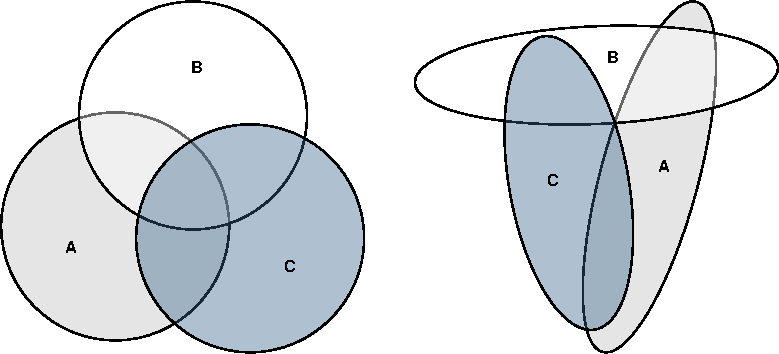
\includegraphics{thesis_files/figure-latex/impossible3-1.pdf}
\caption{\label{fig:impossible3}A set relationship depicted with circles and
ellipses.}
\end{figure}

With four intersecting sets, circular Euler diagrams are actually
impossible, given that \(2^4=16\) regions are required but the circles
can yield at most 14 unique intersections. This is not, however, the
case with ellipses in that they they may intersect in up to 4, rather
than 2, points. All in all, circles have three degrees of freedom:
x-coordinate, y-coordinate, and radius, whereas ellipses have five:
x-coordinate, y-coordinate, semi-minor radius, semi-major radius, and
rotation.

Elliptical Euler diagrams have been successfully implemented in the
\textbf{eulerAPE} software \autocite{micallef_2014}, yet only for three
sets that moreover need to intersect, the motivation for which being
that Euler diagrams with more than three sets often lack adequate
solutions and that their high complexity make implementations difficult
\autocite{micallef_2013}.

As far as we know, analytical solutions to eulerr diagrams do not exist.
All existing implementations are instead based on varying numerical
methods. Most of these use separate methods for the initial and final
diagram configurations. For instance, \textcite{micallef_2013} uses uses
a greedy algorithm, \textcite{wilkinson_2012} uses multi-dimensional
scaling with jacobian distances -- a constrained version of which is
used in \textcite{frederickson_2016} in combination with a greedy
algorithm. The latter two work only on pairwise relationships between
the sets while the first tries to optimize the three-way intersection
between the three sets. All use circles for the initial layout.

Diagrams with more than two sets require additional tuning, which is
considered in a final configuration step. This is always an optimization
procedure with a target loss function and an optimization procedure.

It is this difficulty that we have overcome with \textbf{eulerr}, which
is the first software to provide elliptical Euler diagrams for,
theoretically, any number of sets.

\subsection{Aim}\label{aim}

The aim of this thesis is to present a method and implementation for
constructing and visualizing Euler diagrams for sets of any numbers with
ellipses.

\section{Method}\label{method}

A Euler diagram might be conceived of as a model of data, akin to any
other statistical model. As such, it requires

\begin{itemize}
\tightlist
\item
  some data,
\item
  a process through with which the model is fit,
\item
  a test to check how well it fits, and finally
\item
  a presentation of the result.
\end{itemize}

\subsection{Input}\label{input}

Every Euler diagram begins with data, which, in one way or another, is
always a description of set relationships. \textbf{eulerr} tries to be
as friendly as possible, accepting many forms (Table \ref{tab:data}).

\begin{longtable}[]{@{}ll@{}}
\caption{\label{tab:data} Types of data.}\tabularnewline
\toprule
Form & Example\tabularnewline
\midrule
\endfirsthead
\toprule
Form & Example\tabularnewline
\midrule
\endhead
Named vector & \(A=10 \quad B=5 \quad A \cap B=2\)\tabularnewline
Matrix of logicals or binaries &
\(\begin{bmatrix}\bm{A} & \bm{B} & \bm{C} \\0 & 1 & 0 \\1 & 1 & 1 \\1 & 0 & 0 \\ \end{bmatrix}\)\tabularnewline
A list of sample spaces &
\(\begin{matrix} A = \{ab,\,bb,\,bc\}\\B = \{aa,\,bc,\,cc\}\\C = \{bb,\,bb,\,cc\} \end{matrix}\)\tabularnewline
\bottomrule
\end{longtable}

\subsection{Initial configuration}\label{initial-configuration}

For our initial configuration, we work exclusively with circles. We
begin by mapping the disjoint set combinations to areas and, given
these, figure out the required pairwise distance between the sets to
achieve a circle--circle overlap matching these disjoint set
combinations. We do this numerically, using the formula for a
circle--circle overlap,

\begin{multline}
A = r_1^2\arccos\left(\frac{d^2 + r_1^2 - r_2^2}{2dr_1}\right) + 
r_2^2\arccos\left(\frac{d^2 + r_2^2 - r_1^2}{2dr_2}\right) - \\
\frac{1}{2}\sqrt{(-d + r_1 + r_2)(d + r_1 - r_2)(d - r_1 + r_2)(d + r_1 + r_2)},
\end{multline}

where \(r_1\) and \(r_2\) are the radii of the first and second circles
respectively and \emph{d} the distance between them.

Although \(r_1\) and \(r_2\) are known, \emph{d} is not, wherefore we
approximate it numerically. Here, our loss function is the squared
difference between \emph{A} and the desired overlap, \((A-D)^2\), which
we then ptimize using the \textbf{R}'s built-in \texttt{optimize()}: a
``combination of golden section search and successive parabolic
interpolation.'' Convergence is fast and neglible in relation to our
later, more demanding, operations.

Given these optimal pairwise distances, we can proceed to the next step,
which is to position the circles representing the sets. This can be
accomplished in many ways; \textbf{eulerr} uses a method from the
\textbf{venn.js} script \autocite{frederickson_2016}, namely a
constrained version of multi-dimensional scaling (MDS), which is based
on a similar method from the \textbf{venneuler} package
\autocite{wilkinson_2012}. \textbf{venneuler} tries to place disjoint
and subset exactly neck-in-neck and at the exact midpoint of the set
respectively. However, since we are indifferent about where in the space
outside (or respectively inside) the sets are placed, that behavior
becomes problematic since it might interfere with locations of other
sets that need to use that space.

The MDS algorithm from \textbf{venn.js} circumvents this by assigning a
loss and gradient of 0 when, for instance, the set relationsships
\emph{and} the candidate ellipses are disjoint. Then, to optimize the
pairwise relationsships between sets, \textbf{eulerr} uses the following
loss and gradient functions.

\begin{quote}
\[\small
\text{loss} = \sum_i \sum_j { {\begin{cases}
    0 & \text{disjoint}(i, j)\\ 
    0 & \text{subset}(i, j)\\ 
    ((X_{i} - X_{j})^T(X_{i} - X_{j}) - D_{ij}^2) ^2  & \text{otherwise} \\ 
\end{cases}}}
\]

\[\small
\nabla f(X_{i}) = \sum_j {\begin{cases}
     \vec{0} & \text{disjoint}(i, j)\\ 
     \vec{0} & \text{subset}(i, j)\\ 
     4 {((X_{i} - X_{j})^T(X_{i} - X_{j}) - D_{ij}^2)} (X_{i} -
     X_{j}) & \text{otherwise} \\ 
\end{cases}}\] \emph{Source:
\href{http://www.benfrederickson.com/better-venn-diagrams/}{Better Venn
Diagrams} by Ben Fredrickson, which includes a nice interactive
demonstration.}
\end{quote}

Fredrickson uses the \emph{Polak--Ribière Conjugate Gradient Method} to
optimize the initial layout. In our experience this method occasionally
ends up in local minima, which is why we have opted to use
\texttt{nlm()} from the \textbf{R} core package \texttt{stats}, which is
a translation from FORTRAN code developed by \textcite{schnabel_1985}
and uses a mixture of algorithms (Newton and Quasi-Newton).

This initial configuration will work perfectly for any 1--2 set
combinations and as well as possible with 3 sets if we use circles but
for all other combinations there is usually a need to fine tune the
configuration.

\subsection{Final configuration}\label{final-configuration}

\subsubsection{Intersection between
ellipses}\label{intersection-between-ellipses}

Splitting a conic

\begin{figure}
\centering
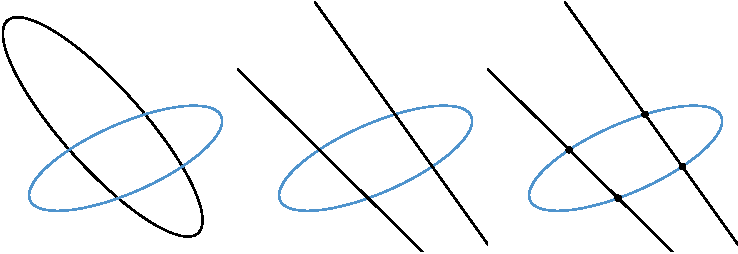
\includegraphics{thesis_files/figure-latex/unnamed-chunk-2-1.pdf}
\caption{\label{fig:unnamed-chunk-2}The process (from left to right) used to
intersect two ellipses, here yielding 4 points.}
\end{figure}

\subsubsection{Areas of overlapping
ellipses}\label{areas-of-overlapping-ellipses}

\subsection{Visualization}\label{visualization}

\section{Results}\label{results}

\subsection{Consistency}\label{consistency}

\subsection{Accuracy}\label{accuracy}

\subsection{Performance}\label{performance}

\section{Discussion}\label{discussion}

\section{Pre-processing}\label{pre-processing}

\section{Initial configuration}\label{initial-configuration-1}

Our initial layout can be setup in a number of ways; \textbf{eulerr}
uses one of the methods from Fredrickson's
\href{https://github.com/benfred/venn.js/}{venn.js}, which features a
constrained version of multi-dimensional scaling (MDS) based on that of
Wilkinson's \textbf{R} package
\href{https://CRAN.R-project.org/package=venneuler}{venneuler}
\autocite{wilkinson_2012}. \textbf{venneuler} tries to place disjoint
and subset exactly neck-in-neck and at the exact midpoint of the set
respectively. However, since we are indifferent about where in the space
outside (or respectively inside) the sets are placed, that behavior
becomes problematic since it might interfere with locations of other
sets that need to occupy some of that space.

The MDS algorithm from \textbf{venn.js} circumvents this by assigning a
loss and gradient of 0 when, for instance, the set relationsships
\emph{and} the candidate ellipses are disjoint. Then, to optimize the
pairwise relationsships between sets, \textbf{eulerr} uses the following
loss and gradient functions.

\begin{quote}
\[\small
\text{loss} = \sum_i \sum_j { {\begin{cases}
    0 & \text{disjoint}(i, j)\\ 
    0 & \text{subset}(i, j)\\ 
    ((X_{i} - X_{j})^T(X_{i} - X_{j}) - D_{ij}^2) ^2  & \text{otherwise} \\ 
\end{cases}}}
\]

\[\small
\nabla f(X_{i}) = \sum_j {\begin{cases}
     \vec{0} & \text{disjoint}(i, j)\\ 
     \vec{0} & \text{subset}(i, j)\\ 
     4 {((X_{i} - X_{j})^T(X_{i} - X_{j}) - D_{ij}^2)} (X_{i} -
     X_{j}) & \text{otherwise} \\ 
\end{cases}}\] \emph{Source:
\href{http://www.benfrederickson.com/better-venn-diagrams/}{Better Venn
Diagrams} by Ben Fredrickson, which includes a nice interactive
demonstration.}
\end{quote}

Fredrickson uses the \emph{Polak--Ribière Conjugate Gradient Method} to
optimize the initial layout. In our experience this method occasionally
ends up in local minima, which is why we have opted to use
\texttt{nlm()} from the \textbf{R} core package \texttt{stats}, which is
a translation from FORTRAN code developed by \textcite{schnabel_1985}
and uses a mixture of algorithms (Newton and Quasi-Newton).

This initial configuration will work perfectly for any 1--2 set
combinations and as well as possible with 3 sets if we use circles but
for all other combinations there is usually a need to fine tune the
configuration.

\section{Final configuration}\label{final-configuration-1}

In order to finalize the configuration we need to be able to compute the
areas of the overlaps of the sets, which as it turns out, is \emph{not}
trivial. In fact, most of methods rely on approximations of the areas
by, for instance, quad-tree binning (\textbf{venneuler}) or polygon
intersections (\textbf{VennMaster} \autocite{kestler_2008}). These
methods yield reasonable estimates but, given that the computation may
have to run for a vast number of iterations, are usually prohibitive in
terms of performance.

\textbf{venn.js} and \textbf{eulerAPE} both, however, use exact
algorithms. Based on the fact that any intersection of ellipses can be
represented as a convex polygon with elliptical segments on the fringes,
it is possible to arrive at exact area calculations.

\subsection{Intersections}\label{intersections}

Finding the areas of the overlaps exactly requires that we first know
the points at which the different ellipses intersect. \textbf{eulerr}'s
approach to this is based on a method outlined by
\textcite{richter-gebert_2011}. \textbf{eulerr} owes significant debt to
the \textbf{R} package \textbf{RConics} \autocite{huber_2014}, which has
been tremendously helpful in developing and, especially, debugging the
algorithm. Some parts of the code are in fact straight-up translations
to C++ from the code in \textbf{RConics}.

The method is based in \emph{projective geometry} (rather than
euclidean). To find the intersection points, the algorithm first

\begin{itemize}
\tightlist
\item
  converts the two ellipses from canonical form to matrix notation. The
  canonical form of a rotated ellipse is given by \[
  \frac{((x-h)\cos(\phi)+(y-k)\sin(\phi))^2}{a^2}+\frac{((x-h) \sin(A)-(y-k)
    \cos(\phi))^2}{b^2} = 1,
  \] where \emph{phi} is the counter-clockwise angle from the positive x
  axis to the semi-major axis \emph{a}. \emph{b} is the semi-minor axis
  whilst \emph{(h, k)} is the center of the ellipse. This is then
  converted to the matrix form \[
  E = \begin{bmatrix}A & B/2 & D/2 \\
                 B/2 & C & E/2 \\
                 D/2 & E/2 & F
  \end{bmatrix},
  \] which may be used to represent any conic. We then
\item
  split one of the ellipses (conics) into a pencil of two lines, and
  subsequently
\item
  intersect the remaining conic with these two lines, which will yield
  between 0 and 4 intersection points.
\end{itemize}

\subsection{Areas}\label{areas}

The next step is to calculate the area of overlap between all the
possible combinations of ellipses. The solution to this was discovered,
as far as I know, by Fredrickson who explains it beautifully in a
\href{http://www.benfrederickson.com/calculating-the-intersection-of-3-or-more-circles/}{blog
post}. It relies on finding all the intersection points between the
currently examined sets that are also within these sets. It is then
trivial to find the area of the convex polygon that these vertices make
up. Finding the rest of the area, which is made up of the ellipse
segments between subsequent points, requires a bit of trigonometry.

Here, we have used an algorithm from \textcite{eberly_area_2016}, which
computes circle integral between the points on the ellipse minus the
area of the triangle made up of the center of the ellipse: \[
A(\theta_0, \theta_1) = F(\theta_1) - F(\theta_1) -
\frac{1}{2}|x_1y_0 - x_0y_1|,
\] \[
\text{where } F(\theta) = \frac{a}{b}\left[ \theta -
\arctan{\left(\frac{(b - a)\sin{2\theta}}{b + a +(b - a )\cos{2\theta}} \right)}
\right]
\]

As our loss function, we use the sum of squared differences between the
disjoint set intersections and the areas we have computed and again use
the \texttt{nlm()} optimizer to layout the set.

This optimization step is the bottleneck of the overall computations in
terms of performance, being that we're optimizing over 5 parameters for
every ellipse (or 3 in the case of circles) -- nevertheless, we're
profitting immensely from the implementation in the C++ programming
language through \textbf{Rcpp} \autocite{eddelbuettel_2011} and its
plugin for the linear algebra library \textbf{Armadillo}
\autocite{eddelbuettel_2014} which ends up making the code much faster
than the java-based \textbf{venneuler}.

\section{Layout}\label{layout}

Since the optimization steps are unconstrained, we run the risk of
ending up with dispersed layouts. To fix this, we use the SKYLINE-BL
rectangle packing algorithm \autocite{jylanki_2010} to pack the disjoint
clusters of ellipses (in case there are any) into a heuristically chosen
bin.

At the time of writing this algorithm is crudely implemented -- for
instance, it does not attempt to rotate the rectangles (boundaries for
the ellipses) or attempt to use. Since we're dealing with a rather
simple version of the rectangle packing problem, however, it seems to do
the trick.

\section{Output}\label{output}

Before we get to plotting the solution, it is useful to know how well
the fit from \textbf{eulerr} matches the input. Sometimes euler diagrams
are just not feasible, particular for combinations with many sets, in
which case we should stop here and look for another design to visualize
the set relationships.

It is not, however, obvious what it means for a euler diagram to ``fit
well''. \textbf{venneuler} uses a metric called \emph{stress}, which is
defined as \[
\frac{\sum_{i=1}^{n} (y_i - \hat{y}_i) ^ 2}{\sum_{i=1}^{n} y_i ^ 2}
\] where \(\hat{y}_i\) is an ordinary least squares estimate from the
regression of the fitted areas on the original areas that is being
explored during optimization.

Meanwhile, \textbf{eulerAPE} \autocite{micallef_2014} uses
\emph{diagError}: \[
\max_{i = 1, 2, \dots, n} \left| \frac{y_i}{\sum y_i} -
  \frac{\hat{y}_i}{\sum \hat{y}_i} \right|
\]

Both metrics are given the user after the diagram has been fit, together
with a table of residuals.

\begin{verbatim}
##       original fitted residuals region_error
## A          1.0  1.038    -0.038        0.021
## B          1.0  1.038    -0.038        0.021
## C          1.0  1.038    -0.038        0.021
## A&B        0.5  0.302     0.198        0.040
## A&C        0.5  0.302     0.198        0.040
## B&C        0.5  0.302     0.198        0.040
## A&B&C      0.0  0.247    -0.247        0.058
## 
## diag_error:  0.058 
## stress:      0.049
\end{verbatim}

\begin{figure}
\centering
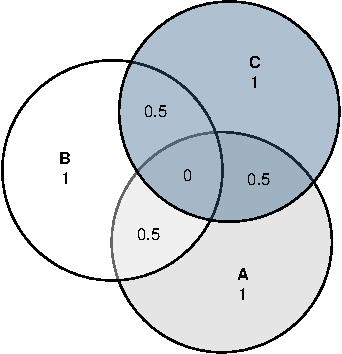
\includegraphics{thesis_files/figure-latex/unnamed-chunk-3-1.pdf}
\caption{\label{fig:unnamed-chunk-3}A plot with circles.}
\end{figure}

It is clear that this is not a good fit, which we can find out just by
looking at the plot. This is a good example of when ellipses come in
handy.

\begin{verbatim}
##       original fitted residuals region_error
## A          1.0    1.0         0            0
## B          1.0    1.0         0            0
## C          1.0    1.0         0            0
## A&B        0.5    0.5         0            0
## A&C        0.5    0.5         0            0
## B&C        0.5    0.5         0            0
## A&B&C      0.0    0.0         0            0
## 
## diag_error:  0 
## stress:      0
\end{verbatim}

\begin{figure}
\centering
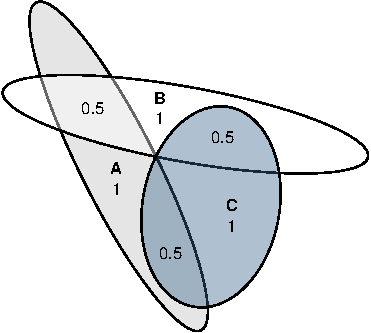
\includegraphics{thesis_files/figure-latex/unnamed-chunk-4-1.pdf}
\caption{\label{fig:unnamed-chunk-4}A plot with ellipses.}
\end{figure}

Much better.

\section{Plotting}\label{plotting}

Let's face it: euler diagrams are naught without visualization. Here,
\textbf{eulerr} interfaces the elegant Lattice graphics system
\autocite{sarkar_2008} to grant the user extensive control over the
output, and allow for facetted plots in case such a design was used in
fitting the euler configuration.

\subsection{Labelling}\label{labelling}

Most users will want to label their euler diagrams. One option is to
simply add a legend

\begin{figure}
\centering
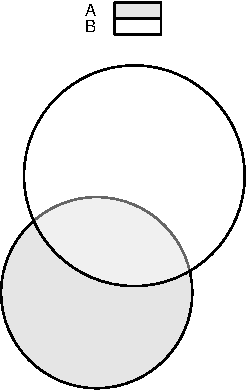
\includegraphics{thesis_files/figure-latex/unnamed-chunk-5-1.pdf}
\caption{\label{fig:unnamed-chunk-5}A simple plot.}
\end{figure}

but many will want to label their diagrams directly, perhaps with
counts.

\begin{figure}
\centering
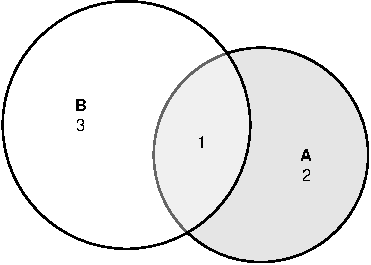
\includegraphics{thesis_files/figure-latex/unnamed-chunk-6-1.pdf}
\caption{\label{fig:unnamed-chunk-6}A plot with counts.}
\end{figure}

In this case, layout out the diagram becomes considerably more involved.
Finding a reasonable spot for the text inside the diagram only lends
itself to an easy solution if the shape of the intersection has a
center-of-gravity inside ellipse, in which case an average of some of
the points might suffice. This is often not the case, however, and we
need a better solution. Specifically, what we need is a method to find
the point inside the circle overlap for the counts and circle complement
to the intersection for our labels.

So far, we have not been able to derive at an analyitcal solution for
finding a good point, or for that matter a reliable way of finding
\emph{any} point that is in the required intersection or complement. As
is often the case, the next-best thing turns out to be a numerical one.
First, we locate a point that is inside the required region by spreading
points across one of the discs involed in the set combination. To spread
points uniformly, we use \emph{Vogel's method}
\autocites{arthur_2015}{vogel_1979} \[
\left( p_k = (\rho_k, \theta_k) = \left( r \sqrt{\frac{k}{n}},\, \pi (3 - \sqrt{5})(k - 1) \right) \right)_{k=1}^n,
\] which is actually based on the golden angle.

\begin{figure}
\centering
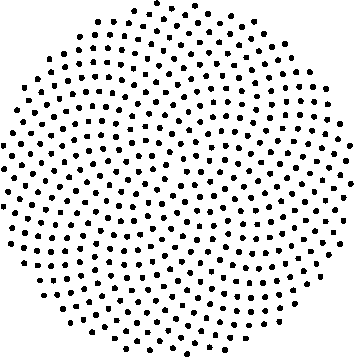
\includegraphics{thesis_files/figure-latex/unnamed-chunk-7-1.pdf}
\caption{\label{fig:unnamed-chunk-7}Spreading points on a disc with Vogel's
method.}
\end{figure}

After this, we scale, translate, and rotate the points so that they fit
the desired ellipse.

After we've spread our points throughout the ellipse and found one that
matches our desired combination of ellipses/sets, we then proceed to
optimize its position numerically. For this, we use version of the
\emph{Nelder--Mead Method} \autocite{nelder_1965} which we've translated
from Matlab code by \textcite{kelley_1999} and customized for
\textbf{eulerr} (in particular to make sure that the simplex does not
escape the intersection boundaries since we for this problem \emph{want}
the local minimum).

\subsection{Coloring}\label{coloring}

Per default, the ellipses are filled with colors. The default option is
to use an adaptive scheme in which colors are chosen to provide a
balance between dinstinctiveness, beauty, and consideration for the
color deficient. The color palette has been generated from
\href{https://CRAN.R-project.org/package=qualpalr}{qualpalr} (developed
by the author), which automatically generates qualitative color palettes
based on a model of color perception.

\printbibliography[title=References]

\end{document}
